\begin{figure}[!htbp]
  \centering
  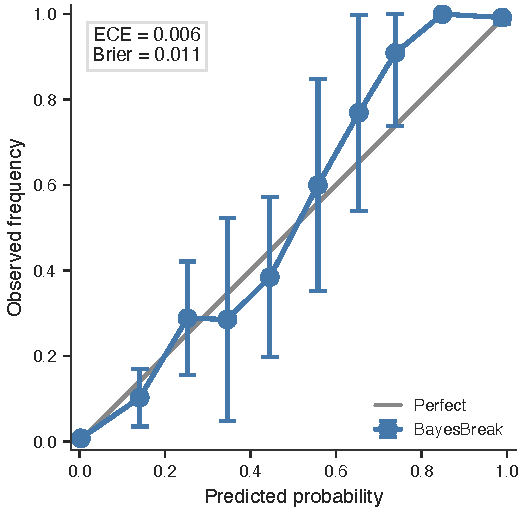
\includegraphics[width=0.78\textwidth,keepaspectratio]{figures/fig3_boundary_calibration.pdf}
  \caption{Calibration of marginal boundary posterior probabilities under synthetic
  Gaussian data (E01, $n=256$, 100 sequences per stratum). The dashed diagonal
  denotes perfect calibration; the curve is the empirical frequency within
  equal-mass bins of predicted posterior boundary probability. Mid-probability
  bins show the most variability because boundary events are intrinsically rare
  per sequence, but the ordering of confidence levels is consistent with
  calibration: bins assigned higher posterior probability correspond to
  higher empirical frequency.}
  \label{fig:calibration}
\end{figure}
